\documentclass{subfiles}
\begin{document}
    \begin{figure}[!h]
        \centering
        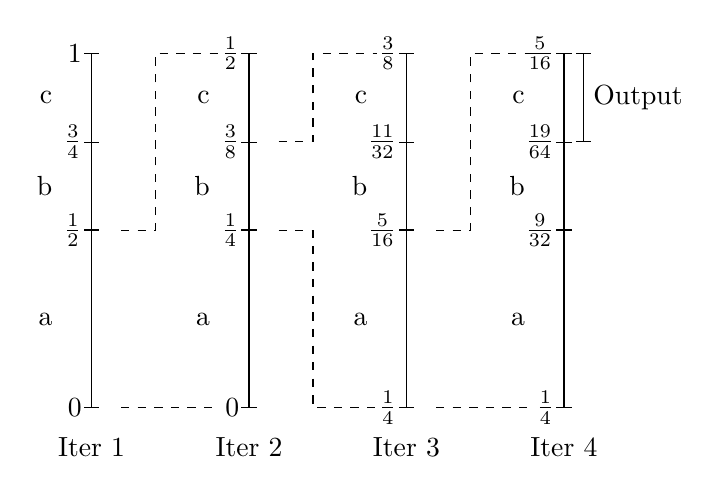
\begin{tikzpicture}
            \foreach \iter in {1, ..., 4}{
                \node at (2*\iter, -0.5) {Iter \iter};
                \draw [ |- ] (2*\iter, 0) -- (2*\iter, 2.25);
                \draw [ |-| ] (2*\iter, 2.25) -- (2*\iter, 3.375);
                \draw [ -| ] (2*\iter, 3.375) -- (2*\iter, 4.5);

                    \node at (2*\iter - 0.25, 1.125) [label=left:a] {};
                    \node at (2*\iter - 0.25, 2.8125) [label=left:b] {};
                    \node at (2*\iter - 0.25, 3.9375) [label=left:c] {};
                }            

            % Iter 1
            \node at (2, 0) [anchor=east] {\(0\)};
            \node at (2, 2.25) [anchor=east] {\(\frac{1}{2}\)};
            \node at (2, 3.375) [anchor=east] {\(\frac{3}{4}\)};
            \node at (2, 4.5) [anchor=east] {\(1\)};

            \draw [dashed] (2.375, 0) -- (3.625, 0);
            \draw [dashed] (2.375, 2.25) -- (2.8125, 2.25) -- (2.8125, 4.5) -- (3.625, 4.5);
        
            % Iter 2
            \node at (4, 0) [anchor=east] {\(0\)};
            \node at (4, 2.25) [anchor=east] {\(\frac{1}{4}\)};
            \node at (4, 3.375) [anchor=east] {\(\frac{3}{8}\)};
            \node at (4, 4.5) [anchor=east] {\(\frac{1}{2}\)};

            \draw [dashed] (4.375, 2.25) -- (4.8125, 2.25) -- (4.8125, 0) -- (5.625, 0);
            \draw [dashed] (4.375, 3.375) -- (4.8125, 3.375) -- (4.8125, 4.5) -- (5.625, 4.5);

            % Iter 3
            \node at (6, 0) [anchor=east] {\(\frac{1}{4}\)};
            \node at (6, 2.25) [anchor=east] {\(\frac{5}{16}\)};
            \node at (6, 3.375) [anchor=east] {\(\frac{11}{32}\)};
            \node at (6, 4.5) [anchor=east] {\(\frac{3}{8}\)}; 

            \draw [dashed] (6.375, 0) -- (7.625, 0);
            \draw [dashed] (6.375, 2.25) -- (6.8125, 2.25) -- (6.8125, 4.5) -- (7.625, 4.5);
            
            % Iter 4
            \node at (8, 0) [anchor=east] {\(\frac{1}{4}\)};
            \node at (8, 2.25) [anchor=east] {\(\frac{9}{32}\)};
            \node at (8, 3.375) [anchor=east] {\(\frac{19}{64}\)};
            \node at (8, 4.5) [anchor=east] {\(\frac{5}{16}\)};

            \draw [ |-| ] (8.25, 3.375) -- (8.25, 4.5);
            \node at (8.25, 3.9375) [anchor=west] {Output};
        \end{tikzpicture}
        \caption{Step by step encoding of \(\omega = abac\) via the \gls{ac}.}
        \label{Fig:3}
    \end{figure}
\end{document}
